%! TEX root = /home/simon/Documents/masterarbete/dagbok/main.tex
\documentclass[swedish, a4paper, 11pt]{report}


%%%%%%%%%%% LANGUAGE %%%%%%%%%%%

% For correct hyphenation in swedish
\usepackage[T1]{fontenc}

% For interpreting non-ASCII characters
\usepackage[utf8]{inputenc}

% International language support
% Fetches language from documentclass options. Most other packages do this as well
\usepackage{babel}


%%%%%%%%%%% FORMAL STUFF %%%%%%%%%%%

% Smaller margins
\usepackage[margin=2.5cm]{geometry}

% Fancy chapter headers
\usepackage{titlesec}
\titleformat{\chapter}{\normalfont\huge}{\thechapter.}{20pt}{\huge\it}

% Dates & time
\usepackage[yyyymmdd]{datetime} % Useful when referencing websites
\renewcommand{\dateseparator}{-} % ISO 8601 date format

% What to display in table of contents
\setcounter{tocdepth}{1}
\setcounter{secnumdepth}{2}

% Lists
\usepackage{enumerate} % Determines the style in which the counter is printed
\usepackage{enumitem} % Provides user control over the layout of the three basic list environments

% Citing & bibliography
\usepackage{csquotes} % For \enquote command for proper quotation marks, also biblatex recommends this
\usepackage[numbers]{natbib}


%%%%%%%%%%% GRAPHICS %%%%%%%%%%%

\usepackage{graphics,color,xcolor}

% Figures
\usepackage{epsfig} % Solves some problems in \includegraphics{<.eps-file>}
\usepackage{graphicx} % More options for \includegraphics
\usepackage{wrapfig} % Figure environment that lets text wrap around figure
\usepackage{float} % Figure placement
\usepackage{caption} % More options for \caption
\usepackage{subcaption} % Subfigures

% Tikz
\usepackage{tikz}
\usepackage{pgf,pgfplots} % Pgfplot
\pgfplotsset{compat=1.15}

% För alduslöv
\usepackage{pifont}


%%%%%%%%%%% PHYSICS %%%%%%%%%%%

% SI units
\usepackage{siunitx}
\DeclareSIUnit\clight{\text{$c$}} % redefine from c_0 to c
\DeclareSIUnit\byte{B}

% Physics macros
\usepackage{physics} % Defines lots of nice commands like \derivative, \norm, \evaluated, etc. It is recommended to use these as much as possible for nice spacing and readable LaTeX code.
\usepackage{braket} % Defines \bra, \ket, \braket, and \set
\usepackage{slashed} % For Feynman slash notation
\usepackage{simpler-wick} % Wick contractions (may require sty-file)
% \usepackage[compat=1.1.0]{tikz-feynman} % Feynman diagrams (has to be compiled with LuaTeX)
\usepackage{tensor} % Covariant index notation


%%%%%%%%%%% CODING %%%%%%%%%%%

% For nice code insertions
\usepackage{listings}
\definecolor{codegreen}{rgb}{0,0.6,0}
\definecolor{codegray}{rgb}{0.5,0.5,0.5}
\definecolor{codepurple}{rgb}{0.58,0,0.82}
\definecolor{backcolour}{rgb}{0.95,0.95,0.92}
\lstdefinestyle{mystyle}{
    backgroundcolor=\color{backcolour},   
    commentstyle=\color{codegreen},
    keywordstyle=\color{magenta},
    numberstyle=\tiny\color{codegray},
    stringstyle=\color{codepurple},
    basicstyle=\ttfamily\footnotesize,
    breakatwhitespace=false,         
    breaklines=true,                 
    captionpos=b,                    
    keepspaces=true,                 
    numbers=left,                    
    numbersep=5pt,                  
    showspaces=false,                
    showstringspaces=false,
    showtabs=false,
    tabsize=4
}
\lstset{style=mystyle}


%%%%%%%%%%% MATHEMATICS %%%%%%%%%%%

% AMS packages
\usepackage{amsmath,amsfonts,amsthm,amssymb}

% Theorem and proof environments
\iflanguage{swedish}{
    \newtheorem{theorem}{Sats}
    \newtheorem*{theorem*}{Sats}
    \newtheorem{proposition}{Proposition}
    \newtheorem*{proposition*}{Proposition}
    \newtheorem{corollary}{Följdsats}[theorem]
    \newtheorem{corollary*}{Följdsats}
    \newtheorem{lemma}{Lemma}
    \newtheorem*{lemma*}{Lemma}
    \theoremstyle{definition}
    \newtheorem{definition}{Definition}
    \newtheorem*{definition*}{Definition}
}{}
\iflanguage{english}{
    \newtheorem{theorem}{Theorem}
    \newtheorem*{theorem*}{Theorem}
    \newtheorem{proposition}{Proposition}
    \newtheorem*{proposition*}{Proposition}
    \newtheorem{corollary}{Corollary}[theorem]
    \newtheorem{corollary*}{Corollary}
    \newtheorem{lemma}{Lemma}
    \newtheorem*{lemma*}{Lemma}
    \theoremstyle{definition}
    \newtheorem{definition}{Definition}
    \newtheorem*{definition*}{Definition}
}{}

% Better version of the \not command
\usepackage{cancel}

 % Does polynomial division for you
\usepackage{polynom}

% Vectors are upright boldface. I think this definition is better than the physics package's \vectorbold.
\let\Vec\undefined % We use \vec w/ lowercase v
\renewcommand*{\vec}[1]{{\boldsymbol{\mathrm{#1}}}}

% Bar, tilde, and hat that scales with what is under them. Basically I just want these to have consistent names
\let\mathbar\overline
\let\mathtilde\widetilde
\let\mathhat\widehat

% Redefine \exp
% Errors occur if this definition is made before some of the packages are loaded
\let\oldexp\exp
\newcommand*{\Exp}[1]{\oldexp{#1}}
\renewcommand{\exp}[1]{\mathrm{e}^{#1}}

% Main number systems
\newcommand{\naturals}{\mathbb{N}}
\newcommand{\integers}{\mathbb{Z}}
\newcommand{\rationals}{\mathbb{Q}}
\newcommand{\reals}{\mathbb{R}}
\newcommand{\compexnumbers}{\mathbb{C}}

% Some of my own shorthands for correct spacing in math environments
\def\divides{\mid} % Proper spacing of vertical bar in division x|y
\def\from{\colon} % Proper spacing of colon in functions f:A→ B
\newlength\mylen % Isomorphic \mapsto
\settowidth\mylen{$\longleftrightarrow$}
\newcommand{\mapsbetween}{\longleftrightarrow\kern - 0.5\mylen\vline height 1.2ex depth -0.0pt\kern0.5\mylen}
\newcommand{\suchthat}{\qq{s.th.}}
\def\definedas{\coloneqq}
\def\defines{\eqqcolon}

\newcommand*{\transpose}[1]{#1^{\!\mathsf{T}}}
\renewcommand*{\complement}[1]{#1^{\mathsf{C}}}
% \newcommand{\conjugate}[1]{\mathbar{#1}}
\newcommand*{\conjugate}[1]{#1^*}
\newcommand*{\hermitianconjugate}[1]{#1^\dag}
\newcommand*{\inverse}[1]{#1^{-1}}

\newcommand*{\closure}[1]{\mathbar{#1}} % Closure of a set
\def\union{\cup}
\newcommand{\Union}{\bigcup\limits}
\def\intersection{\cap}
\newcommand{\Intersection}{\bigcap\limits}

% Lie-groups & algebras, i.g. SU(n)
\newcommand*{\algebra}[2]{\mathfrak{\MakeLowercase{#1}}\left(#2\right)}
\newcommand*{\group}[2]{\mathrm{\MakeUppercase{#1}}\left(#2\right)}


%%%%%%%%%%% MISCELLANEOUS %%%%%%%%%%%

% In-pdf comments through \todo command
\setlength{\marginparwidth}{2cm} % Silence warning about margin size
\usepackage{todonotes}

% Clickable links and refs
\usepackage[hidelinks]{hyperref} 

% Cleverref automatically detects if you are referencing a figure, table, or equation etc
% Cleverref has to be loaded last I think, after babel and hyperref etc
\usepackage[noabbrev, nameinlink]{cleveref}
\crefname{equation}{}{}
\iflanguage{swedish}{ % Tell cleverref to use Oxford comma
	\newcommand{\creflastconjunction}{, och\nobreakspace}
}{}
\iflanguage{english}{
	\newcommand{\creflastconjunction}{, and\nobreakspace}
}{}


% Tag only referenced equations (this is not an ideal package, as it requires etextools, which is buggy and abandoned by its author)
\expandafter\def\csname ver@etex.sty\endcsname{3000/12/31}
\let\globcount\newcount
\usepackage{autonum}

% Intervals on the real line
\let\interval\undefined % To avoid name conflict with etextools
\usepackage{interval}
\intervalconfig{soft open fences}

% For writing \overset{text}&{=} in align environment
\usepackage{aligned-overset} 

\usepackage{textcomp} % Mainly for using interrobang
\synctex=1

\title{{\Huge \ding{166}} Dagbok för masterarbetet {\Huge \ding{166}}}
\author{Simon Stefanus Jacobsson}
\date{2021}

\begin{document}
\renewcommand{\thechapter}{\Roman{chapter}}


\maketitle
\tableofcontents

\chapter{Läsperiod 3}
\section{Vecka 1}
%! TEX root = /home/simon/Documents/Dagbok_MPPHS_2020-2021/main.tex
\subsection{Måndag 2020-11-02}

Ny LP, nya mögligheter. Jag har tre kurser nu, algebraisk geometri, HPC, \& sannolikhetsteori (med Gurra). I geometrin tror jag att Jan Stevens lecture notes är en bra resurs. I HPCn ska jag bara kolla Martin Raums videos och kötta labbar. I sannolikhetsteorin vet jag inte riktigt än vad som är top strat.

Idag vill jag läsa algebraisk geometri på förmiddagen och sen gå på föreläsningar på eftermiddagen.

\bigskip

Föreläsningen i algebraisk geometri var inte superhype. Dock var kurslitteraturen \&så fett kortfattad så vet ej hur jag ska approacha det riktigt. Tänker att jag går bort till Chalmers \& skriver ut kurslitteraturen \& ser om det går att studera utifrån den.

Tagga börja med HPCn imorgon. Gurra sa att han ville sitta och plugga imorgon. Så han kanske får sätta sig här så kan vi göra sannolikhetsteori tsm.

\bigskip

Jag lade till så att jag lägger in \SI{1000}{kr} i månaden i Nordea-fonden.

\subsection{Tisdag 2020-11-03}

Jobbade på helt OK idag. Ska börja med \enquote{Writing to files} i assignment 0 imorgon.


\subsection{Onsdag 2020-11-04}

Fick neovim att fungera på Gantenbein idag :). Fick tillgång till Gantenbein btw. Gurra sa att det var high value att göra inlämningarna på sin egen dator och sen kopiera över dem med \verb+scp+ till Gantenbein.

Satt med Gurra \& gjorde sannolikhetsteori idag. Vi skulle sitta imorgon med sa vi. Men frågan är hur mycket mer jag behöver sitta med sannolikhetsteorin den här veckan. Kanske vill kötta klart ass 0 i HPCn.

Vill läsa klart halva kapitel 1 \& göra uppgifterna i geometrin tills på fredag \&så.


\subsection{Torsdag 2020-11-05}

Hade lite problem imorse med att få GNU debugger (GDB) att fungera, men det löste sig efter att jag följt \href{https://stackoverflow.com/questions/48278881/gdb-complaining-about-missing-raise-c/48287761}{\color{blue}det här} förslaget.

Gjorde klart ass 0 idag. Antar att jag inte behöver lämna in ass 0 och 1 till någon. Vilket är chill.


\subsection{Fredag 2020-11-06}

Jag borde sluta skriva ut i datorsalen på våning 4. Det blir grynigt. Jag tror det brukar bli bättre när jag skriver ut på biblioteket.




% \section{Vecka 2}
% %! TEX root = /home/simon/Documents/Dagbok_MPPHS_2020-2021/main.tex
\subsection{Måndag 2020-11-9}

\verb|let g:loaded_matchparen=1| fungerade för att få neovim att sluta hoppa mellan parenteser på Gantenbein.

\subsection{Tisdag 2020-11-10}

\subsection{Onsdag 2020-11-11}

\subsection{Torsdag 2020-11-12}

\subsection{Fredag 2020-11-13}

\subsection{Lördag 2020-11-14}

Körde HPC hela denna veckan förutom fredagen, då läste jag geometri. Jag har lite grejor kvar jag skulle vilja göra på söndag, bli klar med assignment 1 och se på föreläsningen i sannolikhetsteori.

 En annan sak jag skulle vilja göra framöver är läxorna i geometrin. Tror det är high value för betyget sen också.

\subsection{Söndag 2020-11-15}

Blev klar med ass 1 idag. Imorgon lär det bli sannolikhetsteori hela dagen. Och i övermorgon kanske geometri och fokusera på läxan.


% \section{Vecka 3}
% %! TEX root = /home/simon/Documents/Dagbok_MPPHS_2020-2021/main.tex
\subsection{Måndag 2020-11-16}

\subsection{Tisdag 2020-11-17}

Gjorde hw i geometrin idag. Det kändes bra. Ska nog läsa igenom kapitel 2 imorgon. Det känns som ett rimligt mål.


\subsection{Onsdag 2020-11-18}

Läste igenom kapitel 2 idag och började lite på HW 3. Det kändes lagom. Ska kanske fortsätta med HPC imorgon.


\subsection{Torsdag 2020-11-19}

Repeterade mest algebran idag. Det kändes bra.

Hittade en app, Anki, som gör flash-cards och förhör mig med dem. Det kanske är rätt bra redskap nu i algebran när det är mycket nya begrepp hela tiden. Ska försöka använda lite och se om det känns bra.


\subsection{Fredag 2020-11-20}

Blev typ lite taggad på att köpa ett höj- och sänkbart skrivbord. \href{https://www.ikea.com/se/sv/p/skarsta-skrivbord-sitt-sta-beige-vit-s09320813/}{\color{blue}Det} kostar 2\,200.

Facebook marketplace verkar förövrigt som ett värt ställe att köpa en cykel på. Ska fundera på om jag behöver en bokhylla också.




% \section{Vecka 4}
% %! TEX root = /home/simon/Documents/Dagbok_MPPHS_2020-2021/main.tex
\subsection{Torsdag 2020-11-26}

\verb|hyperfine| som jag använder i hpc:n för att ta tid på saker jag kör i terminalen verkar fett användbart, jag laddar ner det lokalt.

\subsection{Fredag 2020-11-27}
\subsection{Lördag 2020-11-28}
\subsection{Söndag 2020-11-29}


% \section{Vecka 5}
% %! TEX root = /home/simon/Documents/Dagbok_MPPHS_2020-2021/main.tex
\subsection{Måndag 2020-09-28}

Lade till NERDCommenter-pluginet till mitt neovim. Man använder det genom att skriva
\begin{itemize}
	\item \verb|,cc| för att kommentera en/flera rader
	\item \verb|,cu| för att avkommentera en/flera rader.
\end{itemize}

Tänkte försöka skapa ett \enquote{monorepo} med all min kod, som Lindgren. Det blev dock lite whack för jag tänkte skriva en \verb|.gitignore| där jag började med att exkludera allt \& sen inkludera saker efterhand, som en \verb|.gitinclude| liksom, men det verkar som att jag inte kan exkludera filer igen efter det. Om jag skriver\\
\begin{verbatim}
file.txt
!file.txt
file.txt
\end{verbatim}
i min \verb|.gitignore| blir alltså \verb|file.txt| ändå medtaget i repot.

Jag lade alldeles för mycket tid idag på att försöka lösa detta med regex i python. Borde inte lägga mer tid på det.

Asso måndagar överlag brukar mest vara rövningar. Jag kanske ska försöka skippa att vara på föreläsningar på måndagar \& istället bara läsa i boken ellr ngt. Tror det hade varit mer produktivt.

Imorgon ska jag räkna lite uppgifter att lägga upp i \enquote{Renskrivna Demouppgifter} på Canvas. \checkmark


\subsection{Tisdag 2020-09-29}

Inte så strukturerad dag idag, menmen, fick lite kommutativ algebra läst. Fick \&så gjort dom flesta av veckans demouppgifter i TMV157. Ska hålla rövningen på torsdag. Tagga försöka förklara vrf termerna i $\derivative[n]{}{x}f(x) g(x)$ blir Pascals triangel!

Imorgon vill jag nog bara sitta med hw3. Får väl fråga typ Eric Nilsson eller ngn vilka videor som e relevanta om jag inte kan lista ut det sälv.

\bigskip

Fick även ett mail imorse om att systembolaget inte kommer ge ut produktinfo längre via sin API, utan bara butiksinfo. Detta är fett RIP för nu kan Arvid \& jag ju inte på riktigt realisera vår \enquote{efficiently exploring systembolaget}.

\subsection{Onsdag 2020-09-30}

Jag kan SSHa in på min dator även om den sover :) high value info.

\bigskip

TODO: kolla upp de tdär som Elin snackade om om att Chalmers hade samarbete med ngn vårdcentral dit jag skulle kunna gå \& få tips på hur jag ska kunna plugga koncentrerat.

TODO: lämna in arvodesräkning \& deltagarlista efter matlablaben i eftermiddag. \checkmark

Det bästa sättet att signera en PDF i linux är att
\begin{enumerate}
	\item öppna den i Xournal
	\item signera med ritverktyget
	\item File $\blacktriangleright$ Export to PDF
\end{enumerate}

\bigskip

Jag inser nu att jag borde kanske läst HPC istället för standardmodellen... Vet ej om jag vill läsa strängteorin nästa LP heller, men då finns det bara kursen Advanced Simulation and Machine Learning som jag skulle kunna läsa. Hade typ velat göra HPC:n nästa LP. Undra hur bedömningen ser ut i HPC:n, om jag kan läsa den nästa LP \& få den rättad innan året är slut? Antagligen inte.


\subsection{Söndag 2020-10-04}

\begin{itemize}
	\item \verb|zo| för att öppna en section, eller \enquote{fold}, i vim
	\item \verb|zc| för att stänga en section.
\end{itemize}

Jag mailade Martin Raum som håller i HPC:n \& frågade om jag kan göra ursen nästa LP.





% \section{Vecka 6}
% %! TEX root = /home/simon/Documents/Dagbok_MPPHS_2020-2021/main.tex
\subsection{Måndag 2020-10-05}

Ska springa med Kenneth sen idag. Tänker att jag visar honom Safjället \& sen kanske lite utegym.

Han hade dock en deadline så vi sköt upp till onsdag. Men jag gjorde ett event av det i min kalender som jag kunde dela med honom, så nu kommer han inte undan. Safjället any\% speedrun onsdag 7/10 19:00.

\bigskip

Man kan skriva
\begin{verbatim}
	\usepackage{xcolor}
	\pagecolor[rgb]{0,0,0}
	\color[rgb]{0.5,0.5,0.5}
\end{verbatim}
för att få darkmode i sin pdf.

\verb|Tweepy| är en python-wrapper för twitters API, ska ju även finnas någon najjs twitterklient som man kan köra från terminalen :).\verb|Pytrends| är en python-wrapper för googles API.

\bigskip

Robert Berman svarade \& sa att han redan handledde två exjobb. Mailade Bäckdahl igen, ska försöka få till ett möte med honom.

Bäckdahl svarade \& verkade fortfarande taggad så ska ha ett möte med honom onsdag nästa vecka. Tror detta kommer bli bra!

Martin Raum från HPC:n svarade nu \&så \& tyckte inte att det skulle vara några problem att läsa kursen i efterhand. Han gav mig lite tips till \& med :). Jag ska maila Bengt-Erik Mellander för att regga mig på HPC:n snarast.

\bigskip

Vill kanske fortsätta läsa om Hardy-Littlewoods funktion imorgon. Sen kanske maila Jeffrey om \enquote{fixed uniform proportion} på s.\ 92.


\subsection{Tisdag 2020-10-06}

Mailade Bengt-Erik nu \& frågade om han ville anmäla mig till HPC:n. Insåg \&så att jag inte är anmäld till sannolikhetsteorins grunder. Det kanske är lite RIP. Borde typ höra med Bäckdahl vilka kurser han vill att jag ska läsa.

Bengt-Erik sa att kursen var full men att jag kunde maila Joakim Norbeck. Så jag mailade Norbeck \& han reggade mig på kursen :).

Thomas Wernståhl mailade om uppdrag LP2 men jag tror inte jag är super taggad på att ta på mig mer nästa LP asso.


\subsection{Onsdag 2020-10-07}

Fick rätt mycket integrationsteori läst igår, kände mig fett produktiv. Men kanske ska kolla lite på standardmodellen idag då. Kan börja med att kolla igenom hw3 som jag fick tillbaka. \checkmark

Vill kanske börja skriva ner lite bevis i integrationsteorin efter lunch. Kolla om det finns en bevislista. Eventuellt om jag vill kolla på lite subatomärtentor sen.

Det finns nu en bevislista till integrationsteorin,\\
Longer (harder) proofs:
\begin{enumerate}
	\item Theorem 3.20 (Assuming Caratheodory's Theorem 3.25)
	\item Caratheodory's Theorem 3.25
	\item Theorem 3.26 (You do not need to know the proof of Dynkins pi lambda Theorem  although of course you need to know and understand the statement)
	\item Theorem 3.27
	\item Proposition 4.6 
	\item Theorem 4.15
	\item Theorem 5.5 for finite measures (This includes proving Prop. 5.4(i) but not (ii))  (Theorem 5.1 is assumed here.) (Of course by a finite measure, I don't mean that X is finite but only that m(X) is finite.)
	\item Theorem 6.7
	\item Theorem 7.8 for finite measures.
	\item  Theorem 7.9 for finite measures.
	\item  Theorem 8.9
	\item  Theorem 8.10
	\item  Proposition 9.5
\end{enumerate} 
Shorter (Easier) proofs:
\begin{enumerate}
	\item Theorem 3.14
	\item Proposition 3.30
	\item Lemma 3.35
	\item Proposition 4.7 AND 4.8
	\item Corollary 4.16 AND 4.17
	\item Fatou's lemma (assuming the MCT)
	\item The lebesgue dominated convergence Theorem  (assuming Fatou's lemma)
	\item Proposition 4.25
	\item Theorems 4.27 AND 4.28
	\item  Theorem 6.7(i) Only the WLLN
	\item  Proposition 7.10
	\item  Theorem 8.6
\end{enumerate}

\bigskip

Jag skrev till Carlanderska om tån igen.


\subsection{Torsdag 2020-10-08}

Jag hittade \href{http://www.cs.toronto.edu/~tijmen/gnumpyTr.pdf}{\color{blue}en artikel} som beskriver hur man använder gnumpy. Det verkar fett användbart.


\subsection{Fredag 2020-10-09}

Subomtenta idag. Har ej pluggat ngt sedan förra omtentan men tänker att sannolikheten att jag klarar denna tentan är betydligt högre om jag tar den än om jag inte tar den.

Drar till Elins päron ikväll.


% \section{Vecka 7}
% %! TEX root = /home/simon/Documents/Dagbok_MPPHS_2020-2021/main.tex
\subsection{Måndag 2020-10-12}

Börjar dra ihop sig till tents nu. Jag borde fortsätta med att recappa integrationsteorin \& kanske börja recappa algebran \&så.


\subsection{Tisdag 2020-10-13}

Fick limes-3a i subben :).

Vi skriver ner en uppdaterad kursplan:
%! TEX root = /home/simon/Documents/Dagbok_MPPHS_2020-2021/main.tex
\begin{table}[H]
    \centering
    \caption{}
    \label{tab:course_plan_2}
    \begin{tabular}{l|l|l|}
         & Year 1 & Year 2 \\ \hline
        LP1 
        & \begin{tabular}[c]{@{}l@{}}
            \textcolor{compulsory}{Learning from data (C)}\\ \textcolor{compulsory}{Quantum mechanics (B)}\\ \textcolor{compulsory}{Experimental physics (A)}\\ Representation theory
        \end{tabular}
        & \begin{tabular}[c]{@{}l@{}} \textcolor{elective}{Standard model \& beyond (B)}\\ Integration theory\\ Commutative algebra
        \end{tabular} \\ \hline
        LP2
        & \begin{tabular}[c]{@{}l@{}}
            \textcolor{compulsory_elective}{Symmetries (A)}\\ \textcolor{compulsory_elective}{Computational physics (D)}
        \end{tabular}
        & \begin{tabular}[c]{@{}l@{}}
            %\textcolor{elective}{String theory (A)}\\
			\textcolor{elective}{High performance computing}\\
            Algebraic geometry\\
            Sannolikhetsteorins grunder?
        \end{tabular} \\ \hline
        LP3
        & \begin{tabular}[c]{@{}l@{}}
            \textcolor{elective}{Gravitation \& cosmology (A)}\\ Advanced differential calculus
        \end{tabular} &  \\ \hline
        LP4
        & \begin{tabular}[c]{@{}l@{}}
            \textcolor{elective}{Quantum field theory (B)}\\ Vetenskapshistoria (LA)\\ Complex analysis in several variables
        \end{tabular} 
        & \begin{tabular}[c]{@{}l@{}}
            Distributionsteori?
        \end{tabular} \\ \hline
    \end{tabular}
\end{table}


\bigskip

Hade möte med Thomas Bäckdahl nu \& det kändes bra.
Han sa att de mest relevanta kurserna var GR \& diffkalkylen, vilket känns bra nu när jag skippar strängen.
Han sa till \& med att HPC:n nog var fett användbar så känns inte fel att jag tar den nu.
Sammanfattningsvis är idén att jag ska \enquote{undersöka vad som krävs av en rumstid för existens av lösningar till massiva Dirac-ekvationen med hjälp av xAct (\& liknande?) för att hitta irreducibla dekompositioner. Detta baseras på artikeln \enquote{second order symmetry operators}}.

Jag kollade lite \&så på det administrativa \& det verkar inte som att det finns några deadlines. + att Ludde hade inte gjort ngt offeciellt än heller. När det börjar dra ihop sig ska jag skicka in en blankett till
\begin{itemize}
	\item masteransvarig
	\item examinator
	\item instutitionen (MV).
\end{itemize}
Men den mesta infon finns i \verb|Föreskrifter för masterexamensarbeten_2016.pdf|. Annars tänker jag att det jag har att göra nu framöver är att läsa kap.\ 13 i Walds General Relativity som Thomas rekomenderade.


\subsection{torsdag 2020-10-15}

Jag lade hela dagen på att få till ett najjs synthwavetema på vscode. Det blev jättebodgeit \& fungerar bara när jag kör vscode som root. Men det blev fett spaceat
\begin{figure}[H]
	\centering
	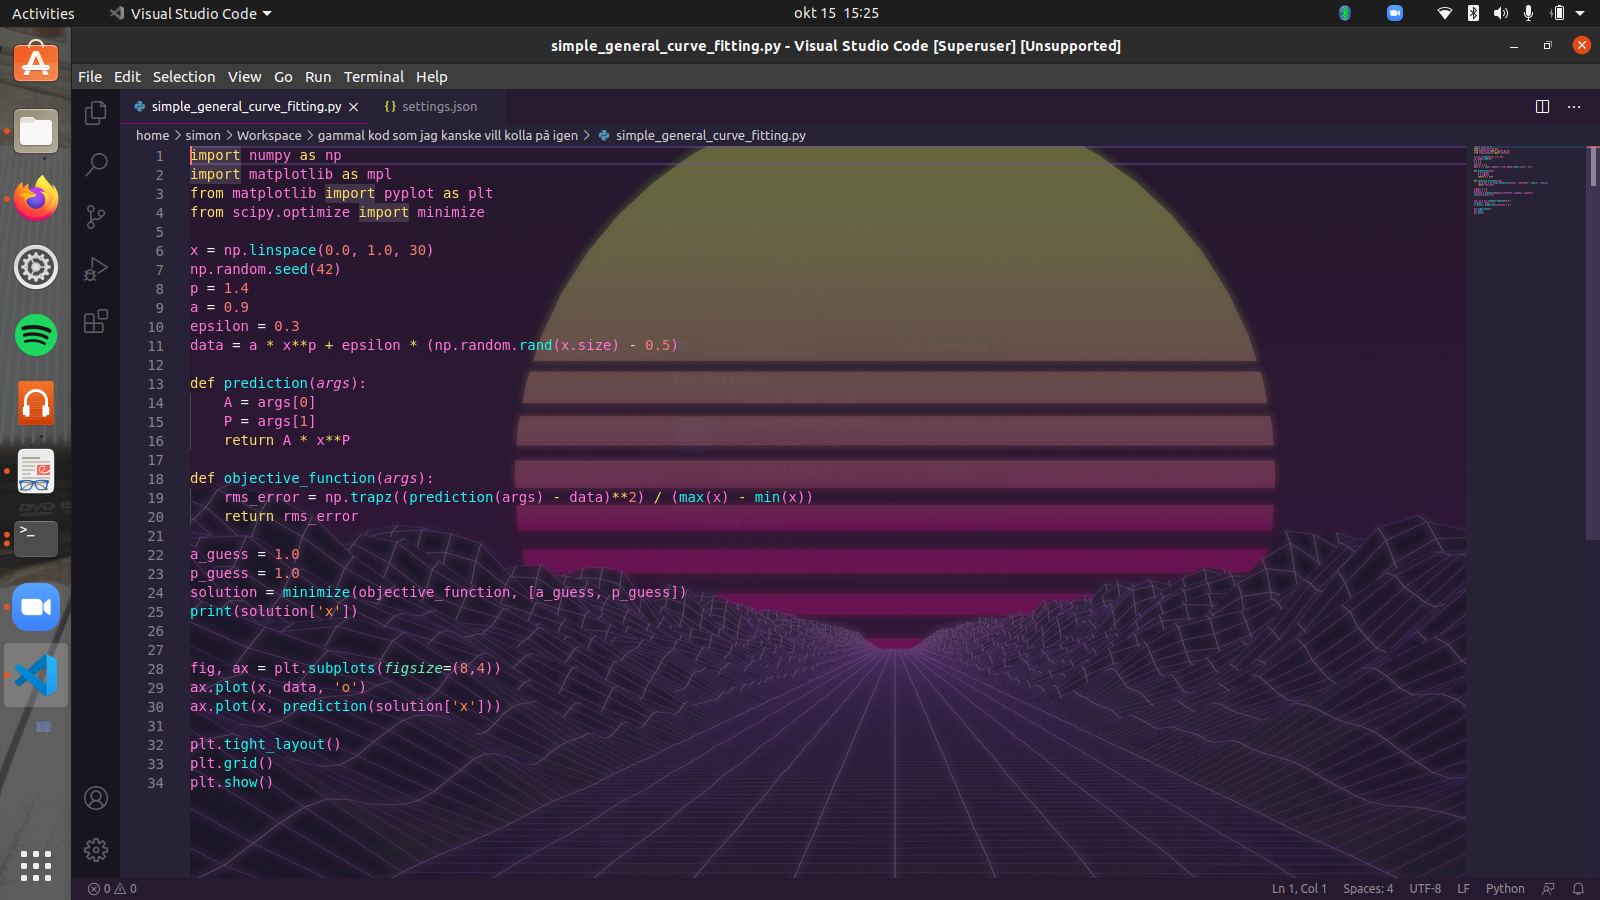
\includegraphics[width=1.0\textwidth]{pics/synthwave_vscode.png}
\end{figure}

Träffade Pontus sen på eftermiddagen \&så, det var fett mysigt. Han berättade bland annat att dom flesta hissar fungerar med relän. det finns alltså ingen mjukvara utan allt är i princip mekaniskt! Även om detta är lite förvånande kan jag se en stor fördel med varför man inte skulle vilja ändå. Det hade inte varit supernajjs om terrorister kunnat hacka hissar.


\subsection{Fredag 2020-10-16}

Lämnade in standardmodellen idag. Hoppas allt e godkännt nu, jag har bodgeat lite med dom två sista inlämningarna. Men om det är det så har jag bara massa integrationsteori \& algebra framför mig. Vilket kommer bli fett hype!

En idé som jag snackade med Eric \& Kevin om idag på lunchen är problemet med om man ska köpa byxor nya eller begagnade.
Om jag köper ett par nya har dom ju inget slitage än så naivt borde man ju tänka att väntevärdet för hur länge dom kommer hålla är större än för ett par begagnade byxor.
Men man måste ju \&så tänka på att om man köper ett par begagnade så är sannolikhetsfördelningen betingad på att dom hållt dittills.
Om $T$ är en slumpvariabel som beskriver hur lång tid ett par byxor håller, så är sannolikheten att de håller en tid $t$, givet att de redan hållt en tid $t_0$, enligt definitionen av betingad sannolikhet
\begin{align}
	P(t \leq T \mid t_0 \leq T) = \frac{P(t \leq T \qq{\&} t_0 \leq T)}{P(t_0 \leq T)} = \begin{cases}
	\frac{P(t \leq T)}{P(t_0 \leq T)} &\qq{om $t_0 \leq t$}\\
	1 &\qq{om $t < t_0$}
	\end{cases}.
\end{align}
Alltså kan man bara ta samma pdf, sätta allt innan $t_0$ till $0$, \& normera.
Vi konstaterade att det kan vara svårt att hitta data på byxor. Eric föreslog att man kanske kan hitta data på hårdiskar.

 


% \section{Vecka 8}
% 
\subsection{Måndag 2020-12-21}
\subsection{Tisdag 2020-12-22}
\subsection{Onsdag 2020-12-23}
\subsection{Torsdag 2020-12-24}
\subsection{Fredag 2020-12-25}
\subsection{Lördag 2020-12-26}
\subsection{Söndag 2020-12-27}




% \section{Tentavecka}
% \input{lp3/Tentavecka}

% \chapter{Läsperiod 4}
% \section{Vecka 1}
% %! TEX root = /home/simon/Documents/Dagbok_MPPHS_2020-2021/main.tex
\subsection{Måndag 2020-11-02}

Ny LP, nya mögligheter. Jag har tre kurser nu, algebraisk geometri, HPC, \& sannolikhetsteori (med Gurra). I geometrin tror jag att Jan Stevens lecture notes är en bra resurs. I HPCn ska jag bara kolla Martin Raums videos och kötta labbar. I sannolikhetsteorin vet jag inte riktigt än vad som är top strat.

Idag vill jag läsa algebraisk geometri på förmiddagen och sen gå på föreläsningar på eftermiddagen.

\bigskip

Föreläsningen i algebraisk geometri var inte superhype. Dock var kurslitteraturen \&så fett kortfattad så vet ej hur jag ska approacha det riktigt. Tänker att jag går bort till Chalmers \& skriver ut kurslitteraturen \& ser om det går att studera utifrån den.

Tagga börja med HPCn imorgon. Gurra sa att han ville sitta och plugga imorgon. Så han kanske får sätta sig här så kan vi göra sannolikhetsteori tsm.

\bigskip

Jag lade till så att jag lägger in \SI{1000}{kr} i månaden i Nordea-fonden.

\subsection{Tisdag 2020-11-03}

Jobbade på helt OK idag. Ska börja med \enquote{Writing to files} i assignment 0 imorgon.


\subsection{Onsdag 2020-11-04}

Fick neovim att fungera på Gantenbein idag :). Fick tillgång till Gantenbein btw. Gurra sa att det var high value att göra inlämningarna på sin egen dator och sen kopiera över dem med \verb+scp+ till Gantenbein.

Satt med Gurra \& gjorde sannolikhetsteori idag. Vi skulle sitta imorgon med sa vi. Men frågan är hur mycket mer jag behöver sitta med sannolikhetsteorin den här veckan. Kanske vill kötta klart ass 0 i HPCn.

Vill läsa klart halva kapitel 1 \& göra uppgifterna i geometrin tills på fredag \&så.


\subsection{Torsdag 2020-11-05}

Hade lite problem imorse med att få GNU debugger (GDB) att fungera, men det löste sig efter att jag följt \href{https://stackoverflow.com/questions/48278881/gdb-complaining-about-missing-raise-c/48287761}{\color{blue}det här} förslaget.

Gjorde klart ass 0 idag. Antar att jag inte behöver lämna in ass 0 och 1 till någon. Vilket är chill.


\subsection{Fredag 2020-11-06}

Jag borde sluta skriva ut i datorsalen på våning 4. Det blir grynigt. Jag tror det brukar bli bättre när jag skriver ut på biblioteket.




% \section{Vecka 2}
% %! TEX root = /home/simon/Documents/Dagbok_MPPHS_2020-2021/main.tex
\subsection{Måndag 2020-11-9}

\verb|let g:loaded_matchparen=1| fungerade för att få neovim att sluta hoppa mellan parenteser på Gantenbein.

\subsection{Tisdag 2020-11-10}

\subsection{Onsdag 2020-11-11}

\subsection{Torsdag 2020-11-12}

\subsection{Fredag 2020-11-13}

\subsection{Lördag 2020-11-14}

Körde HPC hela denna veckan förutom fredagen, då läste jag geometri. Jag har lite grejor kvar jag skulle vilja göra på söndag, bli klar med assignment 1 och se på föreläsningen i sannolikhetsteori.

 En annan sak jag skulle vilja göra framöver är läxorna i geometrin. Tror det är high value för betyget sen också.

\subsection{Söndag 2020-11-15}

Blev klar med ass 1 idag. Imorgon lär det bli sannolikhetsteori hela dagen. Och i övermorgon kanske geometri och fokusera på läxan.


% \section{Påsklov}
% \input{lp4/pasklov}

% \section{Vecka 3}
% %! TEX root = /home/simon/Documents/Dagbok_MPPHS_2020-2021/main.tex
\subsection{Måndag 2020-11-16}

\subsection{Tisdag 2020-11-17}

Gjorde hw i geometrin idag. Det kändes bra. Ska nog läsa igenom kapitel 2 imorgon. Det känns som ett rimligt mål.


\subsection{Onsdag 2020-11-18}

Läste igenom kapitel 2 idag och började lite på HW 3. Det kändes lagom. Ska kanske fortsätta med HPC imorgon.


\subsection{Torsdag 2020-11-19}

Repeterade mest algebran idag. Det kändes bra.

Hittade en app, Anki, som gör flash-cards och förhör mig med dem. Det kanske är rätt bra redskap nu i algebran när det är mycket nya begrepp hela tiden. Ska försöka använda lite och se om det känns bra.


\subsection{Fredag 2020-11-20}

Blev typ lite taggad på att köpa ett höj- och sänkbart skrivbord. \href{https://www.ikea.com/se/sv/p/skarsta-skrivbord-sitt-sta-beige-vit-s09320813/}{\color{blue}Det} kostar 2\,200.

Facebook marketplace verkar förövrigt som ett värt ställe att köpa en cykel på. Ska fundera på om jag behöver en bokhylla också.




% \section{Vecka 4}
% %! TEX root = /home/simon/Documents/Dagbok_MPPHS_2020-2021/main.tex
\subsection{Torsdag 2020-11-26}

\verb|hyperfine| som jag använder i hpc:n för att ta tid på saker jag kör i terminalen verkar fett användbart, jag laddar ner det lokalt.

\subsection{Fredag 2020-11-27}
\subsection{Lördag 2020-11-28}
\subsection{Söndag 2020-11-29}


% \section{Vecka 5}
% %! TEX root = /home/simon/Documents/Dagbok_MPPHS_2020-2021/main.tex
\subsection{Måndag 2020-09-28}

Lade till NERDCommenter-pluginet till mitt neovim. Man använder det genom att skriva
\begin{itemize}
	\item \verb|,cc| för att kommentera en/flera rader
	\item \verb|,cu| för att avkommentera en/flera rader.
\end{itemize}

Tänkte försöka skapa ett \enquote{monorepo} med all min kod, som Lindgren. Det blev dock lite whack för jag tänkte skriva en \verb|.gitignore| där jag började med att exkludera allt \& sen inkludera saker efterhand, som en \verb|.gitinclude| liksom, men det verkar som att jag inte kan exkludera filer igen efter det. Om jag skriver\\
\begin{verbatim}
file.txt
!file.txt
file.txt
\end{verbatim}
i min \verb|.gitignore| blir alltså \verb|file.txt| ändå medtaget i repot.

Jag lade alldeles för mycket tid idag på att försöka lösa detta med regex i python. Borde inte lägga mer tid på det.

Asso måndagar överlag brukar mest vara rövningar. Jag kanske ska försöka skippa att vara på föreläsningar på måndagar \& istället bara läsa i boken ellr ngt. Tror det hade varit mer produktivt.

Imorgon ska jag räkna lite uppgifter att lägga upp i \enquote{Renskrivna Demouppgifter} på Canvas. \checkmark


\subsection{Tisdag 2020-09-29}

Inte så strukturerad dag idag, menmen, fick lite kommutativ algebra läst. Fick \&så gjort dom flesta av veckans demouppgifter i TMV157. Ska hålla rövningen på torsdag. Tagga försöka förklara vrf termerna i $\derivative[n]{}{x}f(x) g(x)$ blir Pascals triangel!

Imorgon vill jag nog bara sitta med hw3. Får väl fråga typ Eric Nilsson eller ngn vilka videor som e relevanta om jag inte kan lista ut det sälv.

\bigskip

Fick även ett mail imorse om att systembolaget inte kommer ge ut produktinfo längre via sin API, utan bara butiksinfo. Detta är fett RIP för nu kan Arvid \& jag ju inte på riktigt realisera vår \enquote{efficiently exploring systembolaget}.

\subsection{Onsdag 2020-09-30}

Jag kan SSHa in på min dator även om den sover :) high value info.

\bigskip

TODO: kolla upp de tdär som Elin snackade om om att Chalmers hade samarbete med ngn vårdcentral dit jag skulle kunna gå \& få tips på hur jag ska kunna plugga koncentrerat.

TODO: lämna in arvodesräkning \& deltagarlista efter matlablaben i eftermiddag. \checkmark

Det bästa sättet att signera en PDF i linux är att
\begin{enumerate}
	\item öppna den i Xournal
	\item signera med ritverktyget
	\item File $\blacktriangleright$ Export to PDF
\end{enumerate}

\bigskip

Jag inser nu att jag borde kanske läst HPC istället för standardmodellen... Vet ej om jag vill läsa strängteorin nästa LP heller, men då finns det bara kursen Advanced Simulation and Machine Learning som jag skulle kunna läsa. Hade typ velat göra HPC:n nästa LP. Undra hur bedömningen ser ut i HPC:n, om jag kan läsa den nästa LP \& få den rättad innan året är slut? Antagligen inte.


\subsection{Söndag 2020-10-04}

\begin{itemize}
	\item \verb|zo| för att öppna en section, eller \enquote{fold}, i vim
	\item \verb|zc| för att stänga en section.
\end{itemize}

Jag mailade Martin Raum som håller i HPC:n \& frågade om jag kan göra ursen nästa LP.





% \section{Vecka 6}
% %! TEX root = /home/simon/Documents/Dagbok_MPPHS_2020-2021/main.tex
\subsection{Måndag 2020-10-05}

Ska springa med Kenneth sen idag. Tänker att jag visar honom Safjället \& sen kanske lite utegym.

Han hade dock en deadline så vi sköt upp till onsdag. Men jag gjorde ett event av det i min kalender som jag kunde dela med honom, så nu kommer han inte undan. Safjället any\% speedrun onsdag 7/10 19:00.

\bigskip

Man kan skriva
\begin{verbatim}
	\usepackage{xcolor}
	\pagecolor[rgb]{0,0,0}
	\color[rgb]{0.5,0.5,0.5}
\end{verbatim}
för att få darkmode i sin pdf.

\verb|Tweepy| är en python-wrapper för twitters API, ska ju även finnas någon najjs twitterklient som man kan köra från terminalen :).\verb|Pytrends| är en python-wrapper för googles API.

\bigskip

Robert Berman svarade \& sa att han redan handledde två exjobb. Mailade Bäckdahl igen, ska försöka få till ett möte med honom.

Bäckdahl svarade \& verkade fortfarande taggad så ska ha ett möte med honom onsdag nästa vecka. Tror detta kommer bli bra!

Martin Raum från HPC:n svarade nu \&så \& tyckte inte att det skulle vara några problem att läsa kursen i efterhand. Han gav mig lite tips till \& med :). Jag ska maila Bengt-Erik Mellander för att regga mig på HPC:n snarast.

\bigskip

Vill kanske fortsätta läsa om Hardy-Littlewoods funktion imorgon. Sen kanske maila Jeffrey om \enquote{fixed uniform proportion} på s.\ 92.


\subsection{Tisdag 2020-10-06}

Mailade Bengt-Erik nu \& frågade om han ville anmäla mig till HPC:n. Insåg \&så att jag inte är anmäld till sannolikhetsteorins grunder. Det kanske är lite RIP. Borde typ höra med Bäckdahl vilka kurser han vill att jag ska läsa.

Bengt-Erik sa att kursen var full men att jag kunde maila Joakim Norbeck. Så jag mailade Norbeck \& han reggade mig på kursen :).

Thomas Wernståhl mailade om uppdrag LP2 men jag tror inte jag är super taggad på att ta på mig mer nästa LP asso.


\subsection{Onsdag 2020-10-07}

Fick rätt mycket integrationsteori läst igår, kände mig fett produktiv. Men kanske ska kolla lite på standardmodellen idag då. Kan börja med att kolla igenom hw3 som jag fick tillbaka. \checkmark

Vill kanske börja skriva ner lite bevis i integrationsteorin efter lunch. Kolla om det finns en bevislista. Eventuellt om jag vill kolla på lite subatomärtentor sen.

Det finns nu en bevislista till integrationsteorin,\\
Longer (harder) proofs:
\begin{enumerate}
	\item Theorem 3.20 (Assuming Caratheodory's Theorem 3.25)
	\item Caratheodory's Theorem 3.25
	\item Theorem 3.26 (You do not need to know the proof of Dynkins pi lambda Theorem  although of course you need to know and understand the statement)
	\item Theorem 3.27
	\item Proposition 4.6 
	\item Theorem 4.15
	\item Theorem 5.5 for finite measures (This includes proving Prop. 5.4(i) but not (ii))  (Theorem 5.1 is assumed here.) (Of course by a finite measure, I don't mean that X is finite but only that m(X) is finite.)
	\item Theorem 6.7
	\item Theorem 7.8 for finite measures.
	\item  Theorem 7.9 for finite measures.
	\item  Theorem 8.9
	\item  Theorem 8.10
	\item  Proposition 9.5
\end{enumerate} 
Shorter (Easier) proofs:
\begin{enumerate}
	\item Theorem 3.14
	\item Proposition 3.30
	\item Lemma 3.35
	\item Proposition 4.7 AND 4.8
	\item Corollary 4.16 AND 4.17
	\item Fatou's lemma (assuming the MCT)
	\item The lebesgue dominated convergence Theorem  (assuming Fatou's lemma)
	\item Proposition 4.25
	\item Theorems 4.27 AND 4.28
	\item  Theorem 6.7(i) Only the WLLN
	\item  Proposition 7.10
	\item  Theorem 8.6
\end{enumerate}

\bigskip

Jag skrev till Carlanderska om tån igen.


\subsection{Torsdag 2020-10-08}

Jag hittade \href{http://www.cs.toronto.edu/~tijmen/gnumpyTr.pdf}{\color{blue}en artikel} som beskriver hur man använder gnumpy. Det verkar fett användbart.


\subsection{Fredag 2020-10-09}

Subomtenta idag. Har ej pluggat ngt sedan förra omtentan men tänker att sannolikheten att jag klarar denna tentan är betydligt högre om jag tar den än om jag inte tar den.

Drar till Elins päron ikväll.


% \section{Vecka 7}
% %! TEX root = /home/simon/Documents/Dagbok_MPPHS_2020-2021/main.tex
\subsection{Måndag 2020-10-12}

Börjar dra ihop sig till tents nu. Jag borde fortsätta med att recappa integrationsteorin \& kanske börja recappa algebran \&så.


\subsection{Tisdag 2020-10-13}

Fick limes-3a i subben :).

Vi skriver ner en uppdaterad kursplan:
%! TEX root = /home/simon/Documents/Dagbok_MPPHS_2020-2021/main.tex
\begin{table}[H]
    \centering
    \caption{}
    \label{tab:course_plan_2}
    \begin{tabular}{l|l|l|}
         & Year 1 & Year 2 \\ \hline
        LP1 
        & \begin{tabular}[c]{@{}l@{}}
            \textcolor{compulsory}{Learning from data (C)}\\ \textcolor{compulsory}{Quantum mechanics (B)}\\ \textcolor{compulsory}{Experimental physics (A)}\\ Representation theory
        \end{tabular}
        & \begin{tabular}[c]{@{}l@{}} \textcolor{elective}{Standard model \& beyond (B)}\\ Integration theory\\ Commutative algebra
        \end{tabular} \\ \hline
        LP2
        & \begin{tabular}[c]{@{}l@{}}
            \textcolor{compulsory_elective}{Symmetries (A)}\\ \textcolor{compulsory_elective}{Computational physics (D)}
        \end{tabular}
        & \begin{tabular}[c]{@{}l@{}}
            %\textcolor{elective}{String theory (A)}\\
			\textcolor{elective}{High performance computing}\\
            Algebraic geometry\\
            Sannolikhetsteorins grunder?
        \end{tabular} \\ \hline
        LP3
        & \begin{tabular}[c]{@{}l@{}}
            \textcolor{elective}{Gravitation \& cosmology (A)}\\ Advanced differential calculus
        \end{tabular} &  \\ \hline
        LP4
        & \begin{tabular}[c]{@{}l@{}}
            \textcolor{elective}{Quantum field theory (B)}\\ Vetenskapshistoria (LA)\\ Complex analysis in several variables
        \end{tabular} 
        & \begin{tabular}[c]{@{}l@{}}
            Distributionsteori?
        \end{tabular} \\ \hline
    \end{tabular}
\end{table}


\bigskip

Hade möte med Thomas Bäckdahl nu \& det kändes bra.
Han sa att de mest relevanta kurserna var GR \& diffkalkylen, vilket känns bra nu när jag skippar strängen.
Han sa till \& med att HPC:n nog var fett användbar så känns inte fel att jag tar den nu.
Sammanfattningsvis är idén att jag ska \enquote{undersöka vad som krävs av en rumstid för existens av lösningar till massiva Dirac-ekvationen med hjälp av xAct (\& liknande?) för att hitta irreducibla dekompositioner. Detta baseras på artikeln \enquote{second order symmetry operators}}.

Jag kollade lite \&så på det administrativa \& det verkar inte som att det finns några deadlines. + att Ludde hade inte gjort ngt offeciellt än heller. När det börjar dra ihop sig ska jag skicka in en blankett till
\begin{itemize}
	\item masteransvarig
	\item examinator
	\item instutitionen (MV).
\end{itemize}
Men den mesta infon finns i \verb|Föreskrifter för masterexamensarbeten_2016.pdf|. Annars tänker jag att det jag har att göra nu framöver är att läsa kap.\ 13 i Walds General Relativity som Thomas rekomenderade.


\subsection{torsdag 2020-10-15}

Jag lade hela dagen på att få till ett najjs synthwavetema på vscode. Det blev jättebodgeit \& fungerar bara när jag kör vscode som root. Men det blev fett spaceat
\begin{figure}[H]
	\centering
	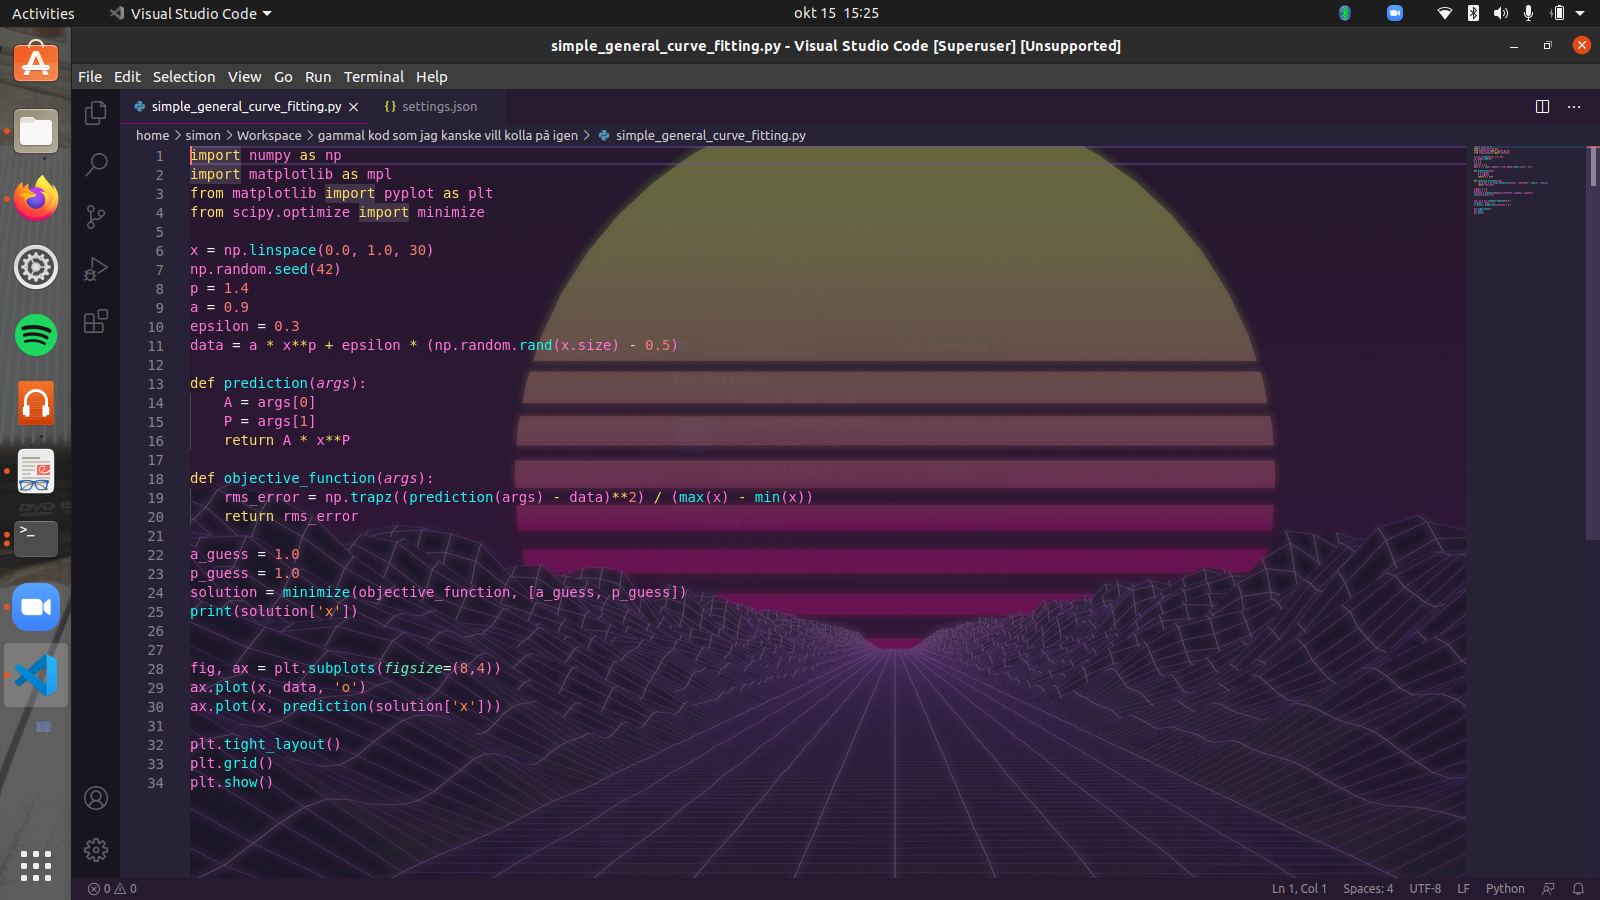
\includegraphics[width=1.0\textwidth]{pics/synthwave_vscode.png}
\end{figure}

Träffade Pontus sen på eftermiddagen \&så, det var fett mysigt. Han berättade bland annat att dom flesta hissar fungerar med relän. det finns alltså ingen mjukvara utan allt är i princip mekaniskt! Även om detta är lite förvånande kan jag se en stor fördel med varför man inte skulle vilja ändå. Det hade inte varit supernajjs om terrorister kunnat hacka hissar.


\subsection{Fredag 2020-10-16}

Lämnade in standardmodellen idag. Hoppas allt e godkännt nu, jag har bodgeat lite med dom två sista inlämningarna. Men om det är det så har jag bara massa integrationsteori \& algebra framför mig. Vilket kommer bli fett hype!

En idé som jag snackade med Eric \& Kevin om idag på lunchen är problemet med om man ska köpa byxor nya eller begagnade.
Om jag köper ett par nya har dom ju inget slitage än så naivt borde man ju tänka att väntevärdet för hur länge dom kommer hålla är större än för ett par begagnade byxor.
Men man måste ju \&så tänka på att om man köper ett par begagnade så är sannolikhetsfördelningen betingad på att dom hållt dittills.
Om $T$ är en slumpvariabel som beskriver hur lång tid ett par byxor håller, så är sannolikheten att de håller en tid $t$, givet att de redan hållt en tid $t_0$, enligt definitionen av betingad sannolikhet
\begin{align}
	P(t \leq T \mid t_0 \leq T) = \frac{P(t \leq T \qq{\&} t_0 \leq T)}{P(t_0 \leq T)} = \begin{cases}
	\frac{P(t \leq T)}{P(t_0 \leq T)} &\qq{om $t_0 \leq t$}\\
	1 &\qq{om $t < t_0$}
	\end{cases}.
\end{align}
Alltså kan man bara ta samma pdf, sätta allt innan $t_0$ till $0$, \& normera.
Vi konstaterade att det kan vara svårt att hitta data på byxor. Eric föreslog att man kanske kan hitta data på hårdiskar.

 


% \section{Vecka 8}
% 
\subsection{Måndag 2020-12-21}
\subsection{Tisdag 2020-12-22}
\subsection{Onsdag 2020-12-23}
\subsection{Torsdag 2020-12-24}
\subsection{Fredag 2020-12-25}
\subsection{Lördag 2020-12-26}
\subsection{Söndag 2020-12-27}




% \section{Vecka 9}
% %! TEX root = /home/simon/Documents/Dagbok_MPPHS_2020-2021/main.tex
\subsection{Måndag 2020-10-26}

Skrev tentan i kommutativ algebra idag. Det gick skitdåligt. Jag lämnade inte in något. Sen byggde jag dator med Kenneth.


\subsection{Tisdag 2020-10-27}

\href{https://github.com/s-n-ushakov/rename-efi-entry}{\color{blue}Här} är ett najjs script för att byta namn på entries i UEFI boot manager.

\subsection{Onsdag 2020-10-28}

Hade integrationsteorimunta idag. Det kändes helt OK även om jag inte kom ihåg allt. Jeff sa att jag var godkännd iaf.

Jag installerade KVM/QEMU för att köra virtuel machines på min dator. Jag kan mounta en .iso \& köra den genom
\begin{verbatim}
qemu-img create -f qcow2 testing_manjaro.img 10G
qemu-system-x86_64 -m 2048 -boot d -enable-kvm -smp 2 -net nic -net user -hda
    testing_manjaro.img -cdrom Downloads/manjaro-xfce-20.1.2-201019-linux58.iso
\end{verbatim}
Jag hittade en najjs \href{https://fosspost.org/use-qemu-test-operating-systems-distributions/}{\color{blue}källa} som förklarade lite om hur man kör QEMU. Den ger en förklaring till ovanstående kommandon:
\begin{figure}[H]
	\centering
	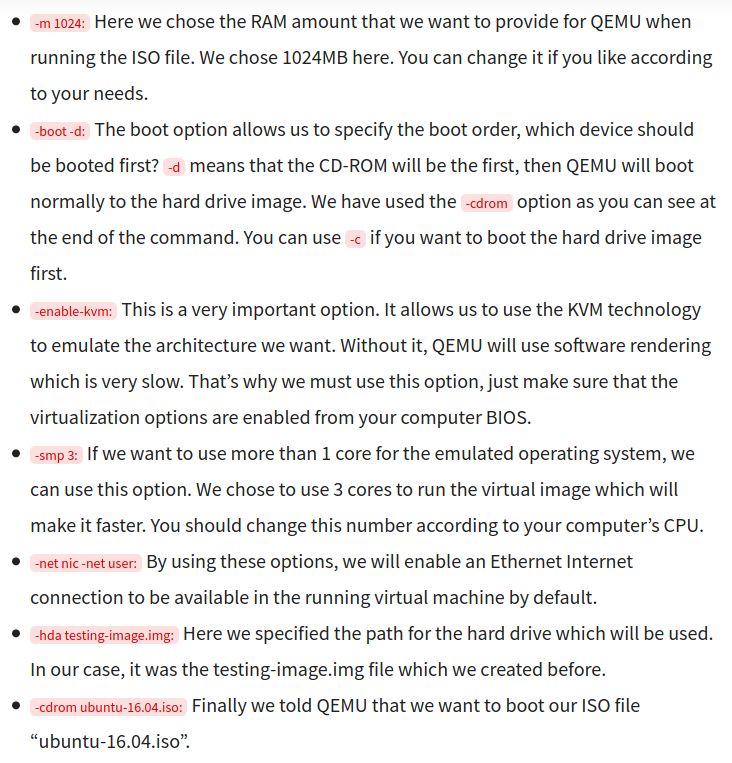
\includegraphics[width=0.8\textwidth]{pics/qemu_explained_example.png}
\end{figure}
Sen efter jag installerat kan jag köra
\begin{verbatim}
qemu-system-x86_64 -m 2048 -boot d -enable-kvm -smp 2 -net nic -net user -hda
    testing_manjaro.img
\end{verbatim}
för att starta det installerade operativsystemet :).




% \section{Vecka 10}
% \input{lp4/v10}

\bibliographystyle{aipauth4-1}
% \nocite{aipauth42Control}
\bibliography{bibliography} % A file named bibliography.bib containing the bibTeX entries should be placed beside the main.tex file

\end{document}
